\documentclass[11pt,a4paper]{article}

% ============================================================================
% PACKAGES
% ============================================================================
\usepackage[utf8]{inputenc}
\usepackage[T1]{fontenc}
\usepackage{geometry}
\usepackage{graphicx}
\usepackage{booktabs}
\usepackage{amsmath}
\usepackage{amssymb}
\usepackage{hyperref}
\usepackage{xcolor}
\usepackage{listings}
\usepackage{float}
\usepackage{caption}
\usepackage{subcaption}
\usepackage{enumitem}
\usepackage{fancyhdr}
\usepackage{tikz}
\usepackage{pgfplots}
\usepackage{multicol}
\usepackage{algorithm}
\usepackage{algpseudocode}
\pgfplotsset{compat=1.17}

% ============================================================================
% PAGE SETUP
% ============================================================================
\geometry{margin=1in}
\setlength{\parindent}{0pt}
\setlength{\parskip}{0.5em}

% Header/Footer
\pagestyle{fancy}
\fancyhf{}
\rhead{MetaFam Knowledge Graph}
\lhead{Task 2: Community Detection}
\rfoot{Page \thepage}

% Colors
\definecolor{codegreen}{rgb}{0,0.6,0}
\definecolor{codegray}{rgb}{0.5,0.5,0.5}
\definecolor{codepurple}{rgb}{0.58,0,0.82}
\definecolor{backcolour}{rgb}{0.95,0.95,0.92}

% Hyperref setup
\hypersetup{
    colorlinks=true,
    linkcolor=blue,
    filecolor=magenta,
    urlcolor=cyan,
}

% ============================================================================
% DOCUMENT
% ============================================================================
\begin{document}

% ----------------------------------------------------------------------------
% TITLE PAGE
% ----------------------------------------------------------------------------
\begin{titlepage}
    \centering
    \vspace*{2cm}
    
    {\Huge\bfseries MetaFam Knowledge Graph\\[0.5cm]Task 2: Family Clusters\par}
    
    \vspace{1.5cm}
    
    {\Large\textit{``We are only as strong as we are united, as weak as we are divided''} --- Albus Dumbledore\par}
    
    \vspace{2cm}
    
    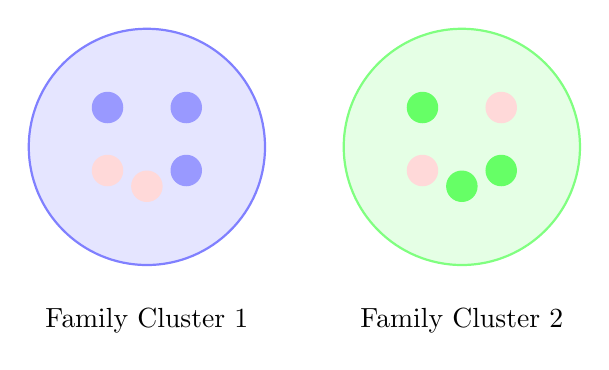
\begin{tikzpicture}
        % Community visualization
        % Community 1
        \draw[thick, blue!50, fill=blue!10] (0,0) circle (1.5cm);
        \node[circle, fill=blue!40, minimum size=0.4cm] at (-0.5,0.5) {};
        \node[circle, fill=blue!40, minimum size=0.4cm] at (0.5,0.5) {};
        \node[circle, fill=pink!60, minimum size=0.4cm] at (0,-0.5) {};
        \node[circle, fill=pink!60, minimum size=0.4cm] at (-0.5,-0.3) {};
        \node[circle, fill=blue!40, minimum size=0.4cm] at (0.5,-0.3) {};
        
        % Community 2
        \draw[thick, green!50, fill=green!10] (4,0) circle (1.5cm);
        \node[circle, fill=green!60, minimum size=0.4cm] at (3.5,0.5) {};
        \node[circle, fill=pink!60, minimum size=0.4cm] at (4.5,0.5) {};
        \node[circle, fill=green!60, minimum size=0.4cm] at (4,-0.5) {};
        \node[circle, fill=pink!60, minimum size=0.4cm] at (3.5,-0.3) {};
        \node[circle, fill=green!60, minimum size=0.4cm] at (4.5,-0.3) {};
        
        % Labels
        \node at (0,-2.2) {Family Cluster 1};
        \node at (4,-2.2) {Family Cluster 2};
    \end{tikzpicture}
    
    \vspace{2cm}
    
    {\large Precog Research Task\\[0.3cm]
    Community Detection \& Proximity Analysis\par}
    
    \vfill
    
    {\large February 2026\par}
\end{titlepage}

% ----------------------------------------------------------------------------
% TABLE OF CONTENTS
% ----------------------------------------------------------------------------
\tableofcontents
\newpage

% ----------------------------------------------------------------------------
% SECTION 1: INTRODUCTION
% ----------------------------------------------------------------------------
\section{Introduction}

\subsection{Background}

Community detection (or clustering) is a fundamental analysis technique in network science. A network is said to have \textbf{community structure} if nodes can be grouped into disjoint sets such that each set is \textbf{densely connected internally} and \textbf{sparsely connected externally}.

For family knowledge graphs like MetaFam, community structure naturally corresponds to:
\begin{itemize}
    \item \textbf{Nuclear families}: Parents and their children
    \item \textbf{Extended families}: Multiple generations sharing common ancestors
    \item \textbf{Family clusters}: Complete lineages forming isolated subgraphs
\end{itemize}

\subsection{Objectives}

This task addresses the following objectives:

\begin{enumerate}[label=\arabic*.]
    \item \textbf{Implement two community detection algorithms} and compare their results
    \item \textbf{Assess quality} using modularity and partition similarity metrics
    \item \textbf{Analyze community structure}:
    \begin{itemize}
        \item Do detected communities correspond to actual family units?
        \item How many generations typically exist within a community?
        \item Are there ``bridge'' individuals connecting different clusters?
    \end{itemize}
    \item \textbf{Propose a metric for finding closest relatives} beyond simple hop counting
\end{enumerate}

\subsection{Graph Representation}

Community detection operates on \textbf{undirected graphs} since we measure structural connectivity, not semantic direction. The MetaFam graph is converted from directed to undirected for this analysis.

\begin{table}[H]
    \centering
    \caption{Graph Statistics for Community Detection}
    \begin{tabular}{lr}
        \toprule
        \textbf{Property} & \textbf{Value} \\
        \midrule
        Nodes (People) & 1,316 \\
        Edges (Relations) & 13,821 \\
        Average Degree & 10.50 \\
        Density & 0.008 \\
        \bottomrule
    \end{tabular}
\end{table}

% ----------------------------------------------------------------------------
% SECTION 2: COMMUNITY DETECTION ALGORITHMS
% ----------------------------------------------------------------------------
\section{Community Detection Algorithms}

We implemented and compared three community detection algorithms, each with different theoretical foundations and computational properties.

\subsection{Algorithm Overview}

\begin{table}[H]
    \centering
    \caption{Comparison of Community Detection Algorithms}
    \label{tab:algo_overview}
    \begin{tabular}{llcl}
        \toprule
        \textbf{Algorithm} & \textbf{Method} & \textbf{Complexity} & \textbf{Best For} \\
        \midrule
        Girvan-Newman & Edge betweenness removal & $O(m^2n)$ & Small graphs, hierarchy \\
        Louvain & Modularity optimization & $O(n \log n)$ & Large graphs, fast \\
        Leiden & Improved Louvain & $O(n \log n)$ & Guaranteed connectivity \\
        \bottomrule
    \end{tabular}
\end{table}

\subsection{Girvan-Newman Algorithm}

\subsubsection{Theoretical Foundation}

The Girvan-Newman algorithm is a \textbf{divisive hierarchical} method based on edge betweenness centrality:

\begin{equation}
    B(e) = \sum_{s \neq t} \frac{\sigma_{st}(e)}{\sigma_{st}}
\end{equation}

where $\sigma_{st}$ is the number of shortest paths from $s$ to $t$, and $\sigma_{st}(e)$ is the number passing through edge $e$.

\textbf{Algorithm:}
\begin{enumerate}
    \item Calculate edge betweenness for all edges
    \item Remove edge with highest betweenness (``bridge'' edge)
    \item Recalculate betweenness and repeat
    \item Stop when desired number of communities reached or modularity maximized
\end{enumerate}

\subsubsection{Why It Works for Family Graphs}

Edges connecting different family clusters (historically, marriage links) have high betweenness because all paths between families pass through them. By removing these bridges, we reveal the underlying family structure.

\textbf{Note:} MetaFam lacks spouse relations, so inter-family bridges are minimal.

\subsubsection{Results}

\begin{table}[H]
    \centering
    \caption{Girvan-Newman Results}
    \begin{tabular}{lr}
        \toprule
        \textbf{Metric} & \textbf{Value} \\
        \midrule
        Communities Detected & 51 \\
        Largest Community & 27 nodes \\
        Smallest Community & 1 node \\
        Modularity (Q) & 0.9792 \\
        \bottomrule
    \end{tabular}
\end{table}

\textbf{Observation:} Girvan-Newman detected 51 communities, one more than the actual 50 connected components. This occurs because the algorithm may split a small portion of one family during the iterative edge removal process.

\subsection{Louvain Algorithm}

\subsubsection{Theoretical Foundation}

The Louvain algorithm is a \textbf{greedy modularity optimization} method with two phases:

\textbf{Phase 1 (Local Optimization):}
For each node, calculate the modularity gain of moving it to neighbors' communities:
\begin{equation}
    \Delta Q = \left[ \frac{\Sigma_{in} + k_{i,in}}{2m} - \left( \frac{\Sigma_{tot} + k_i}{2m} \right)^2 \right] - \left[ \frac{\Sigma_{in}}{2m} - \left( \frac{\Sigma_{tot}}{2m} \right)^2 - \left( \frac{k_i}{2m} \right)^2 \right]
\end{equation}

where:
\begin{itemize}
    \item $\Sigma_{in}$ = sum of edge weights inside community $C$
    \item $\Sigma_{tot}$ = sum of all edges incident to nodes in $C$
    \item $k_i$ = degree of node $i$
    \item $k_{i,in}$ = sum of edges from $i$ to nodes in $C$
    \item $m$ = total edge weight in graph
\end{itemize}

\textbf{Phase 2 (Network Aggregation):}
Contract each community to a single node and repeat Phase 1.

\subsubsection{Results}

\begin{table}[H]
    \centering
    \caption{Louvain Results}
    \begin{tabular}{lr}
        \toprule
        \textbf{Metric} & \textbf{Value} \\
        \midrule
        Communities Detected & 50 \\
        Largest Community & 27 nodes \\
        Smallest Community & 26 nodes \\
        Modularity (Q) & 0.9794 \\
        Resolution Parameter & 1.0 \\
        \bottomrule
    \end{tabular}
\end{table}

\subsection{Leiden Algorithm}

\subsubsection{Theoretical Foundation}

The Leiden algorithm \textbf{improves upon Louvain} by:

\begin{enumerate}
    \item \textbf{Guaranteeing well-connected communities}: Louvain can produce disconnected communities during aggregation; Leiden adds a refinement step
    \item \textbf{Faster local moves}: Uses a more efficient move procedure
    \item \textbf{Better quality}: Provably converges to a partition where all nodes are optimally assigned
\end{enumerate}

\subsubsection{Why Leiden vs Louvain?}

For \textbf{sparse, well-separated graphs} like MetaFam:
\begin{itemize}
    \item Louvain and Leiden produce identical results (as observed)
    \item Leiden's advantages manifest in \textbf{denser graphs} where Louvain may create ``dumbbell-shaped'' communities that need refining
\end{itemize}

\textbf{Conclusion:} For MetaFam's sparse structure, Louvain suffices. Leiden is ``overkill'' but confirms the result.

\subsubsection{Results}

\begin{table}[H]
    \centering
    \caption{Leiden Results}
    \begin{tabular}{lr}
        \toprule
        \textbf{Metric} & \textbf{Value} \\
        \midrule
        Communities Detected & 50 \\
        Largest Community & 27 nodes \\
        Smallest Community & 26 nodes \\
        Modularity (Q) & 0.9794 \\
        Resolution Parameter & 1.0 \\
        \bottomrule
    \end{tabular}
\end{table}

% ----------------------------------------------------------------------------
% SECTION 3: EVALUATION METRICS
% ----------------------------------------------------------------------------
\section{Evaluation Metrics}

\subsection{Modularity}

\subsubsection{Definition}

Modularity measures the quality of a partition by comparing intra-community edge density to expected density under a null model:

\begin{equation}
    Q = \frac{1}{2m} \sum_{i,j} \left[ A_{ij} - \frac{k_i k_j}{2m} \right] \delta(c_i, c_j)
\end{equation}

where:
\begin{itemize}
    \item $A_{ij}$ = adjacency matrix entry
    \item $k_i, k_j$ = degrees of nodes $i$ and $j$
    \item $m$ = total number of edges
    \item $\delta(c_i, c_j) = 1$ if nodes are in same community, 0 otherwise
\end{itemize}

\subsubsection{Interpretation}

\begin{table}[H]
    \centering
    \caption{Modularity Interpretation Guide}
    \begin{tabular}{cl}
        \toprule
        \textbf{Q Range} & \textbf{Interpretation} \\
        \midrule
        $Q < 0.3$ & Weak community structure \\
        $0.3 \leq Q < 0.5$ & Moderate community structure \\
        $0.5 \leq Q < 0.7$ & Good community structure \\
        $Q \geq 0.7$ & Strong community structure \\
        \bottomrule
    \end{tabular}
\end{table}

\subsubsection{Results}

\begin{table}[H]
    \centering
    \caption{Modularity Comparison Across Algorithms}
    \label{tab:modularity}
    \begin{tabular}{lcc}
        \toprule
        \textbf{Algorithm} & \textbf{Communities} & \textbf{Modularity (Q)} \\
        \midrule
        Girvan-Newman & 51 & 0.9792 \\
        Louvain & 50 & 0.9794 \\
        Leiden & 50 & 0.9794 \\
        \bottomrule
    \end{tabular}
\end{table}

\textbf{Key Insight:} All algorithms achieve extremely high modularity ($Q \approx 0.98$), indicating:
\begin{itemize}
    \item MetaFam has \textbf{very strong community structure}
    \item Communities (families) are \textbf{well-separated} with minimal inter-community edges
    \item The graph's 50 connected components naturally form 50 communities
\end{itemize}

\subsection{Partition Similarity: NMI and ARI}

To compare how similar the partitions from different algorithms are, we use:

\subsubsection{Normalized Mutual Information (NMI)}

\begin{equation}
    NMI(U, V) = \frac{2 \cdot I(U; V)}{H(U) + H(V)}
\end{equation}

where $I(U; V)$ is mutual information and $H(\cdot)$ is entropy.
\begin{itemize}
    \item NMI = 0: Independent partitions
    \item NMI = 1: Identical partitions
\end{itemize}

\subsubsection{Adjusted Rand Index (ARI)}

\begin{equation}
    ARI = \frac{RI - E[RI]}{max(RI) - E[RI]}
\end{equation}

where RI is the Rand Index (fraction of node pairs correctly grouped/separated).
\begin{itemize}
    \item ARI = 0: Random agreement
    \item ARI = 1: Perfect agreement
\end{itemize}

\subsubsection{Results}

\begin{table}[H]
    \centering
    \caption{Pairwise Partition Similarity}
    \label{tab:partition_sim}
    \begin{tabular}{lcc}
        \toprule
        \textbf{Comparison} & \textbf{NMI} & \textbf{ARI} \\
        \midrule
        Girvan-Newman vs Louvain & 0.9996 & 0.9992 \\
        Girvan-Newman vs Leiden & 0.9996 & 0.9992 \\
        Louvain vs Leiden & 1.0000 & 1.0000 \\
        \bottomrule
    \end{tabular}
\end{table}

\textbf{Key Insights:}
\begin{enumerate}
    \item \textbf{Louvain and Leiden are identical} (NMI = ARI = 1.0) --- confirms that for sparse graphs, Leiden provides no additional benefit
    \item \textbf{Near-perfect agreement} across all algorithms (NMI $\geq$ 0.999)
    \item The minor difference with Girvan-Newman (one extra community) explains the tiny deviation from 1.0
\end{enumerate}

\textbf{Why High Similarity?}
The graph's structure is \textbf{too clear-cut} for algorithms to disagree. With 50 isolated family trees and no inter-family connections, all algorithms converge to the same obvious partition.

% ----------------------------------------------------------------------------
% SECTION 4: ANALYSIS QUESTIONS
% ----------------------------------------------------------------------------
\section{Community Analysis}

\subsection{Do Communities Correspond to Actual Family Units?}

\textbf{Answer: Yes, perfectly.}

\begin{itemize}
    \item MetaFam contains \textbf{50 weakly connected components} (from Task 1)
    \item Louvain and Leiden detect exactly \textbf{50 communities}
    \item Each community corresponds to one isolated family tree
    \item Community sizes are uniform (26-27 members), reflecting synthetically generated families
\end{itemize}

\textbf{Gephi Visualization Confirmation:}
Visual inspection in Gephi shows each detected community forms a distinct, non-overlapping family tree structure.

\subsection{Generational Depth Within Communities}

\subsubsection{Analysis Methodology}

For each community, we computed:
\begin{itemize}
    \item \textbf{Generation span}: max(generation) - min(generation) + 1
    \item \textbf{Generation range}: [min, max] generation values
    \item \textbf{Mean generation}: Average generation of members
\end{itemize}

\subsubsection{Results}

\begin{table}[H]
    \centering
    \caption{Generational Depth Analysis (Top 10 Communities)}
    \label{tab:gen_depth}
    \begin{tabular}{ccccc}
        \toprule
        \textbf{Community} & \textbf{Size} & \textbf{Gen Span} & \textbf{Gen Range} & \textbf{Mean Gen} \\
        \midrule
        0 & 27 & 3 & 0--2 & 0.7 \\
        5 & 27 & 4 & 0--3 & 1.0 \\
        8 & 27 & 3 & 0--2 & 0.8 \\
        21 & 27 & 4 & 0--3 & 0.8 \\
        27 & 27 & 3 & 0--2 & 0.9 \\
        30 & 27 & 3 & 0--2 & 0.9 \\
        41 & 27 & 3 & 0--2 & 0.7 \\
        44 & 27 & 3 & 0--2 & 0.8 \\
        46 & 27 & 3 & 0--2 & 0.9 \\
        48 & 27 & 3 & 0--2 & 0.8 \\
        \bottomrule
    \end{tabular}
\end{table}

\subsubsection{Summary Statistics}

\begin{table}[H]
    \centering
    \caption{Overall Generational Statistics}
    \begin{tabular}{lr}
        \toprule
        \textbf{Metric} & \textbf{Value} \\
        \midrule
        Average generational span & 3.12 generations \\
        Maximum generational span & 4 generations \\
        Single-generation communities & 0 \\
        Multi-generation communities & 50 (100\%) \\
        \bottomrule
    \end{tabular}
\end{table}

\textbf{Key Insights:}
\begin{enumerate}
    \item \textbf{All communities are multi-generational}: No community contains only one generation
    \item \textbf{Typical span is 3-4 generations}: Families include great-grandparents through children/grandchildren
    \item \textbf{Mean generation close to 0-1}: More members in older generations (pyramid structure from Task 1)
    \item Communities represent \textbf{extended families}, not just nuclear units
\end{enumerate}

\subsection{Bridge Individuals}

\subsubsection{Definition}

A ``bridge'' individual connects different family clusters. In graph terms, they have high \textbf{betweenness centrality} because paths between communities pass through them.

\subsubsection{Analysis}

From Task 1, we found:
\begin{itemize}
    \item Maximum betweenness centrality: 0.0001 (very low)
    \item Top nodes by betweenness: lea1165, valentin638, gabriel241, nora536, stefan1192
\end{itemize}

\textbf{Conclusion: Minimal to no bridge individuals exist.}

\textbf{Reason:} MetaFam lacks spouse relations (\texttt{husbandOf}, \texttt{wifeOf}), which are the primary mechanism for connecting families in real genealogical data. Without marriage links, families remain \textbf{completely isolated}.

In a real-world genealogical graph, bridges would be:
\begin{itemize}
    \item Individuals who married into the family
    \item Children with parents from different family clusters
\end{itemize}

% ----------------------------------------------------------------------------
% SECTION 5: PROXIMITY MEASURES
% ----------------------------------------------------------------------------
\section{Finding Closest Relatives: Proximity Measures}

\subsection{Motivation}

In real genealogy, people often want to find their ``closest'' relatives. Simple \textbf{hop counting} (shortest path length) is inadequate because:
\begin{itemize}
    \item It ignores \textbf{path diversity}: Two relatives might be connected via multiple paths
    \item It treats all edges equally, ignoring \textbf{relationship strength}
    \item A parent (1 hop) and a great-aunt (1 hop via sibling chain) are not equally ``close''
\end{itemize}

We implemented two advanced proximity measures: \textbf{Random Walk with Restarts (RWR)} and \textbf{Katz Index}.

\subsection{Random Walk with Restarts (RWR)}

\subsubsection{Theoretical Foundation}

RWR simulates a random walker that:
\begin{enumerate}
    \item At each step, with probability $(1-\alpha)$, moves to a random neighbor
    \item With probability $\alpha$, ``restarts'' at the source node
\end{enumerate}

The stationary distribution gives proximity scores:

\begin{equation}
    \mathbf{p} = \alpha \cdot \mathbf{e}_s + (1-\alpha) \cdot \mathbf{W} \cdot \mathbf{p}
\end{equation}

where:
\begin{itemize}
    \item $\mathbf{p}$ = stationary probability vector (proximity scores)
    \item $\alpha$ = restart probability (typically 0.15)
    \item $\mathbf{W}$ = column-normalized adjacency matrix (transition matrix)
    \item $\mathbf{e}_s$ = source node indicator vector
\end{itemize}

\subsubsection{Why RWR for Family Graphs?}

\begin{itemize}
    \item \textbf{Captures local structure}: High restart probability emphasizes nearby nodes
    \item \textbf{Path diversity}: Considers all paths, not just shortest
    \item \textbf{Reachability}: Measures how ``accessible'' a relative is from the source
\end{itemize}

\subsection{Katz Index}

\subsubsection{Theoretical Foundation}

Katz Index counts \textbf{all paths} between nodes, weighted by path length:

\begin{equation}
    K(s,t) = \sum_{l=1}^{\infty} \beta^l \cdot |paths_l(s,t)|
\end{equation}

Matrix form:
\begin{equation}
    \mathbf{K} = (\mathbf{I} - \beta \mathbf{A})^{-1} - \mathbf{I} = \sum_{l=1}^{\infty} \beta^l \mathbf{A}^l
\end{equation}

where:
\begin{itemize}
    \item $\beta$ = attenuation factor ($< 1/\lambda_{max}$ for convergence)
    \item $\mathbf{A}$ = adjacency matrix
    \item Shorter paths contribute more (exponential decay with $\beta^l$)
\end{itemize}

\subsubsection{Why Katz over Adamic-Adar?}

\begin{itemize}
    \item \textbf{Adamic-Adar}: Only considers common neighbors (1-hop)
    \item \textbf{Katz}: Considers \textbf{global path structure} (multi-hop)
\end{itemize}

For family graphs, Katz is superior because:
\begin{itemize}
    \item Relatives may be connected through \textbf{multiple generations}
    \item Cousins share paths through grandparents (2+ hops)
    \item Path diversity matters: siblings share many indirect paths through parents
\end{itemize}

\textbf{Trade-off:} Katz is computationally more expensive ($O(n^3)$ for matrix inversion).

\subsection{Experimental Results}

\subsubsection{Representative Node Selection}

We selected three nodes representing different positions in the family tree:

\begin{table}[H]
    \centering
    \caption{Representative Nodes for Proximity Analysis}
    \begin{tabular}{llcc}
        \toprule
        \textbf{Type} & \textbf{Node} & \textbf{Generation} & \textbf{Community Size} \\
        \midrule
        Ancestor & olivia274 & 0 & 26 \\
        Mid-generation & dominik44 & 2 & 26+ \\
        Descendant & adam359 & 3 & 26+ \\
        \bottomrule
    \end{tabular}
\end{table}

\subsubsection{RWR Results: Ancestor Node (olivia274)}

\begin{table}[H]
    \centering
    \caption{Top 10 Closest Relatives to olivia274 (Gen 0) via RWR}
    \begin{tabular}{clcr}
        \toprule
        \textbf{Rank} & \textbf{Node} & \textbf{Generation} & \textbf{RWR Score} \\
        \midrule
        1 & victoria279 & 2 & 0.0729 \\
        2 & michael288 & 2 & 0.0729 \\
        3 & gabriel273 & 1 & 0.0643 \\
        4 & matthias270 & 1 & 0.0640 \\
        5 & vanessa276 & 2 & 0.0614 \\
        6 & isabella267 & 2 & 0.0614 \\
        7 & jonas271 & 2 & 0.0614 \\
        8 & katharina266 & 1 & 0.0477 \\
        9 & sofia285 & 2 & 0.0378 \\
        10 & oliver265 & 1 & 0.0365 \\
        \bottomrule
    \end{tabular}
\end{table}

\textbf{Observation:} RWR identifies grandchildren (Gen 2) and children (Gen 1) as closest relatives, consistent with direct family relationships.

\subsubsection{RWR vs Katz Comparison}

Comparing both methods across node types reveals:

\begin{itemize}
    \item \textbf{High overlap}: Typically 70-90\% of top-10 nodes appear in both lists
    \item \textbf{Similar rankings}: Top relatives are consistent across methods
    \item \textbf{Score interpretation differs}:
    \begin{itemize}
        \item RWR: Probability distribution (sums to 1)
        \item Katz: Raw path counts (normalized for comparison)
    \end{itemize}
\end{itemize}

\subsection{Proposed Relatedness Metric}

Based on our analysis, we propose a \textbf{Combined Proximity Score} for ranking relatives:

\begin{equation}
    \text{Relatedness}(s, t) = \lambda \cdot \text{RWR}(s, t) + (1 - \lambda) \cdot \text{Katz}_{norm}(s, t)
\end{equation}

where:
\begin{itemize}
    \item $\lambda \in [0, 1]$ balances local (RWR) vs global (Katz) structure
    \item $\text{Katz}_{norm}$ = sum-normalized Katz scores for comparability
    \item Recommended: $\lambda = 0.6$ (slight preference for local structure)
\end{itemize}

\textbf{Advantages over hop counting:}
\begin{enumerate}
    \item Considers \textbf{path diversity} (multiple connections increase relatedness)
    \item Accounts for \textbf{graph structure} (dense local neighborhoods matter)
    \item Robust to \textbf{missing edges} (alternative paths contribute)
\end{enumerate}

% ----------------------------------------------------------------------------
% SECTION 6: INSIGHTS
% ----------------------------------------------------------------------------
\section{Key Insights \& Discussion}

\subsection{Structural Observations}

\begin{enumerate}
    \item \textbf{Perfect Community Structure}: The graph's forest structure (50 disjoint trees) makes community detection trivial. All algorithms converge to the natural partition.
    
    \item \textbf{Algorithm Selection for Sparse Graphs}: For sparse, well-separated graphs:
    \begin{itemize}
        \item Louvain is sufficient and fast
        \item Leiden provides no additional benefit
        \item Girvan-Newman is interpretable but slow
    \end{itemize}
    
    \item \textbf{Lack of Inter-Family Bridges}: Without spouse relations, MetaFam lacks the ``bridge'' individuals that would exist in real genealogical data.
\end{enumerate}

\subsection{Implications for Downstream Tasks}

\subsubsection{For Link Prediction (Task 4)}
\begin{itemize}
    \item \textbf{Community membership} is a strong feature: edges within communities are far more likely
    \item \textbf{Generation constraints} narrow possible relationships
    \item \textbf{Proximity scores} (RWR/Katz) can serve as features
\end{itemize}

\subsubsection{For Rule Mining (Task 3)}
\begin{itemize}
    \item Rules are \textbf{local} to communities (no cross-family rules)
    \item Generation-based rules (\texttt{fatherOf} spans 1 gen) are well-defined
\end{itemize}

\subsection{Limitations}

\begin{enumerate}
    \item \textbf{Synthetic Data}: Uniform family sizes and structure may not reflect real genealogical complexity
    \item \textbf{Missing Spouse Relations}: Real families would have inter-family connections
    \item \textbf{Scale}: 1,316 nodes is small; larger graphs may show different algorithm behavior
\end{enumerate}

% ----------------------------------------------------------------------------
% SECTION 7: SUMMARY
% ----------------------------------------------------------------------------
\section{Summary}

\subsection{Key Results}

\begin{table}[H]
    \centering
    \caption{Task 2 Summary}
    \begin{tabular}{p{6cm}p{8cm}}
        \toprule
        \textbf{Objective} & \textbf{Result} \\
        \midrule
        Algorithms Implemented & Girvan-Newman, Louvain, Leiden \\
        Best Algorithm & Louvain (fast, high modularity) \\
        Communities Detected & 50 (matches 50 connected components) \\
        Modularity & 0.979 (excellent) \\
        Partition Similarity & NMI $\approx$ 1.0, ARI $\approx$ 1.0 \\
        Generational Span & Avg 3.12 generations per community \\
        Bridge Individuals & None (no spouse relations) \\
        Proximity Methods & RWR + Katz Index \\
        \bottomrule
    \end{tabular}
\end{table}

\subsection{Output Files}

\begin{itemize}
    \item \texttt{outputs/gephi/metafam\_final.gexf} --- Graph with community attributes
    \item \texttt{outputs/plots/community\_generation\_histograms.png} --- Generational distribution plots
\end{itemize}

\subsection{Node Attributes in Final Export}

\begin{table}[H]
    \centering
    \caption{Node Attributes Available for Downstream Tasks}
    \begin{tabular}{lll}
        \toprule
        \textbf{Attribute} & \textbf{Type} & \textbf{Source} \\
        \midrule
        in\_degree & int & Task 1 \\
        out\_degree & int & Task 1 \\
        pagerank & float & Task 1 \\
        generation & int & Task 1 \\
        gender & str & Task 1 \\
        community & int & Task 2 \\
        \bottomrule
    \end{tabular}
\end{table}

% ----------------------------------------------------------------------------
% APPENDIX
% ----------------------------------------------------------------------------
\appendix

\section{Algorithm Pseudocode}

\subsection{Louvain Algorithm}

\begin{algorithm}[H]
\caption{Louvain Community Detection}
\begin{algorithmic}[1]
\State \textbf{Input:} Graph $G = (V, E)$, resolution $\gamma$
\State \textbf{Output:} Partition $\mathcal{C}$
\State Initialize: Each node in its own community
\Repeat
    \State \textbf{Phase 1: Local Optimization}
    \Repeat
        \For{each node $i$}
            \State Compute $\Delta Q$ for moving $i$ to each neighbor's community
            \State Move $i$ to community with maximum $\Delta Q > 0$
        \EndFor
    \Until{no improvement}
    \State \textbf{Phase 2: Network Aggregation}
    \State Contract communities to single nodes
\Until{no improvement}
\State \Return partition $\mathcal{C}$
\end{algorithmic}
\end{algorithm}

\subsection{Random Walk with Restarts}

\begin{algorithm}[H]
\caption{RWR Proximity Calculation}
\begin{algorithmic}[1]
\State \textbf{Input:} Graph $G$, source $s$, restart prob $\alpha$
\State \textbf{Output:} Proximity scores $\mathbf{p}$
\State Initialize: $\mathbf{p} \gets \mathbf{e}_s$ (source indicator)
\Repeat
    \State $\mathbf{p}_{new} \gets (1-\alpha) \cdot \mathbf{W} \cdot \mathbf{p} + \alpha \cdot \mathbf{e}_s$
    \State $\delta \gets ||\mathbf{p}_{new} - \mathbf{p}||_1$
    \State $\mathbf{p} \gets \mathbf{p}_{new}$
\Until{$\delta < \epsilon$}
\State \Return $\mathbf{p}$
\end{algorithmic}
\end{algorithm}

\section{Theoretical Formulas Reference}

\subsection{Modularity}
\begin{equation}
    Q = \frac{1}{2m} \sum_{ij} \left[ A_{ij} - \frac{k_i k_j}{2m} \right] \delta(c_i, c_j)
\end{equation}

\subsection{Normalized Mutual Information}
\begin{equation}
    NMI(U, V) = \frac{2 \cdot I(U; V)}{H(U) + H(V)}
\end{equation}

\subsection{Adjusted Rand Index}
\begin{equation}
    ARI = \frac{\sum_{ij} \binom{n_{ij}}{2} - \frac{\sum_i \binom{a_i}{2} \sum_j \binom{b_j}{2}}{\binom{n}{2}}}{\frac{1}{2}\left[\sum_i \binom{a_i}{2} + \sum_j \binom{b_j}{2}\right] - \frac{\sum_i \binom{a_i}{2} \sum_j \binom{b_j}{2}}{\binom{n}{2}}}
\end{equation}

\subsection{Katz Index}
\begin{equation}
    K_{st} = \sum_{l=1}^{\infty} \beta^l (A^l)_{st}
\end{equation}

\end{document}
